\documentclass{standalone}
\usepackage{tikz}  %TikZ central library is called.
\usetikzlibrary{automata,positioning} 
\tikzset{%
  every neuron/.style={
    circle,
    draw,
    minimum size=0.8cm
  },
  neuron missing/.style={
    draw=none, 
    scale=2,
    text height=0.2cm,
    execute at begin node=\color{black}$\vdots$
  }
 }

\begin{document}
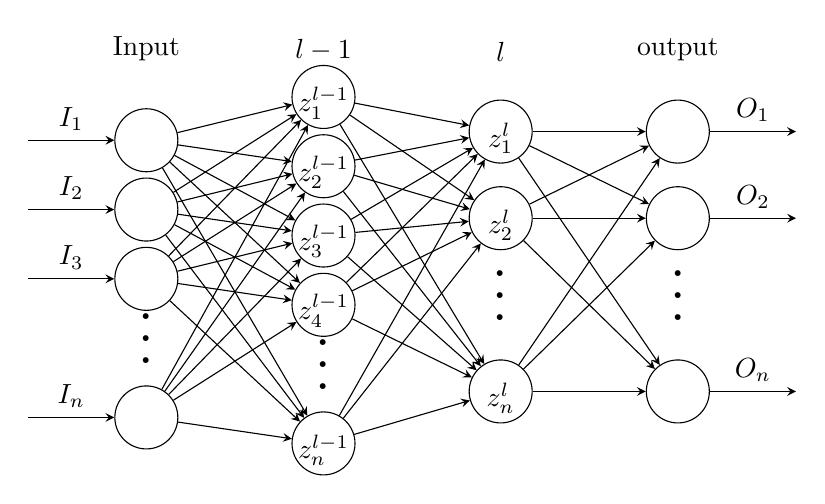
\begin{tikzpicture}[x=1.5cm, y=1.1cm, >=stealth]

\foreach \m/\l [count=\y] in {1,2,3,missing,4}
  \node [every neuron/.try, neuron \m/.try] (input-\m) at (0, 2-\y*0.8) {};

\foreach \m [count=\y] in {1, 2, 3, 4, missing, 5}
  \node [every neuron/.try, neuron \m/.try ] (hiddenl-\m) at (1.5, 2.5-\y*0.8) {};
  
\foreach \m [count=\y] in {1, 2, missing, 3}
  \node [every neuron/.try, neuron \m/.try ] (hidden-\m) at (3, 2.3-\y) {};
  
\foreach \m [count=\y] in {1,2, missing, 3}
  \node [every neuron/.try, neuron \m/.try ] (output-\m) at (4.5,2.3-\y) {};

\foreach \l [count=\i] in {1,2,3, n}
  \draw [<-] (input-\i) -- ++(-1,0)
    node [above, midway] {$I_\l$};

\foreach \l [count=\i] in {1, 2, 3, 4, n}
  \node [above] at (hiddenl-\i.south) {$z^{l-1}_\l$};

\foreach \l [count=\i] in {1, 2, n}
  \node [above] at (hidden-\i.south) {$z^{l}_\l$};
  
\foreach \l [count=\i] in {1,2, n}
  \draw [->] (output-\i) -- ++(1,0)
    node [above, midway] {$O_\l$};

\foreach \i in {1,...,4}
  \foreach \j in {1,...,5}
    \draw [->] (input-\i) -- (hiddenl-\j);
    
\foreach \i in {1,...,5}
  \foreach \j in {1,...,3}
    \draw [->] (hiddenl-\i) -- (hidden-\j);
    
\foreach \i in {1,...,3}
  \foreach \j in {1,...,3}
    \draw [->] (hidden-\i) -- (output-\j);

\foreach \l [count=\x from 0] in {Input, $l-1$, $l$, output}
  \node [align=center, above] at (\x*1.5,2) {\l};

\end{tikzpicture}

\end{document}


